
%%%%%%%%%%%%%%%%%%%%%%%%%%%%%%%%%%%%%%%%%%%%%%%%%%%%%%%%%%%%%%%%%%%%%%%%%%%%%%
%%% Preamble

%%% Document Type
\documentclass[11pt]{article}

%%% Packages
\usepackage{amsmath,amssymb,cancel,units} % math environment and symbols
\usepackage{array}                        % for better arrays (eg matrices) in maths
\usepackage{paralist}                     % very flexible & customisable lists (eg. enumerate/itemize, etc.)
\usepackage{verbatim}                     % adds environment for commenting out blocks of text & for better verbatim
\usepackage[pdftex,bookmarks,colorlinks,breaklinks]{hyperref}  % PDF hyperlinks, with coloured links
\usepackage{memhfixc}                     % remove conflict between the memoir class & hyperref
\usepackage{graphicx}                     % Add graphics capabilities
\usepackage{xspace}                        % smart space insertion after commands
\usepackage{tabulary}
\usepackage{listings}
\usepackage[table]{xcolor} % http://tex.stackexchange.com/questions/5363/how-to-create-alternating-rows-in-a-table

%%% Notation and Variables

\newcommand{\targetData}{D}
\newcommand{\trainingData}[1]{D^{*#1}}
\newcommand{\modelCategory}[1]{M_{#1}}
\newcommand{\modelCategories}{\mathbf{M}}

%%%%%%%%%%%%%%%%%%%%%%%%%%%%%%%%%%%%%%%%%%%%%%%%%%%%%%%%%%%%%%%%%%%%%%%%%%%%%%%
%% Main Document
\begin{document}
% \rowcolors{2}{gray!25}{gray!15}

\title{ARCHIPELAGO}
\author{Jeet Sukumaran}
\maketitle

\section{Introduction}

``Archipelago'' is the name of a generative phylogeny-based model that simultaneously incorporates the diversification processes of speciation and extinction nad the biogeographical processes of area gain (``dispersal'') and area loss (``extirpation''), with these processes being differentially regulated by ecological or other traits that are themselves co-evolving on the phylogeny.
The theory and background to this model and its usage is described in the following paper:


This software project, ``archipelago'' presents a suite of programs to generate and analyze data under the Archipelago model.
The primary objective of the analysis is \textit{model selection}: i.e., statistically identifying the model that generated a particular set of data.
% to \textit{classify a dataset with respect to the model that generated it}.
``archipelago'' is, thus, a computational biogeographical model selection analysis package that exploits the power and flexibility of the Archipelago model to allow you to ask and answer historical biogeographical questions of a nature and complexity that are not possible under any other approach.
In particular, instead of asking questions about ancestral area patterns, you can ask questions about processes, and how some processes (e.g., ecology) affect other processes (e.g., dispersal or speciation).

\section{Installation}

\subsection{Pre-requisites}

\begin{itemize}
    \item Python 2.7 or higher
    \item DendroPy Phylogenetic Computing Library, version 4 or above (\url{http://dendropy.org}).
    \item R (\url{http://www.r-project.org/})
    \item The following R packages:
    \begin{itemize}
        \item adegenet
        \item picante
        \item BioGeoBears
        \item GEIGER
    \end{itemize}
\end{itemize}

\subsection{Installation from Source}

Run the following in the top-level directory of the project:

\begin{lstlisting}
    python setup.py install
\end{lstlisting}


\section{Usage}

\section{Overview of Workflow}

\begin{figure}[h!]
    \begin{center}
        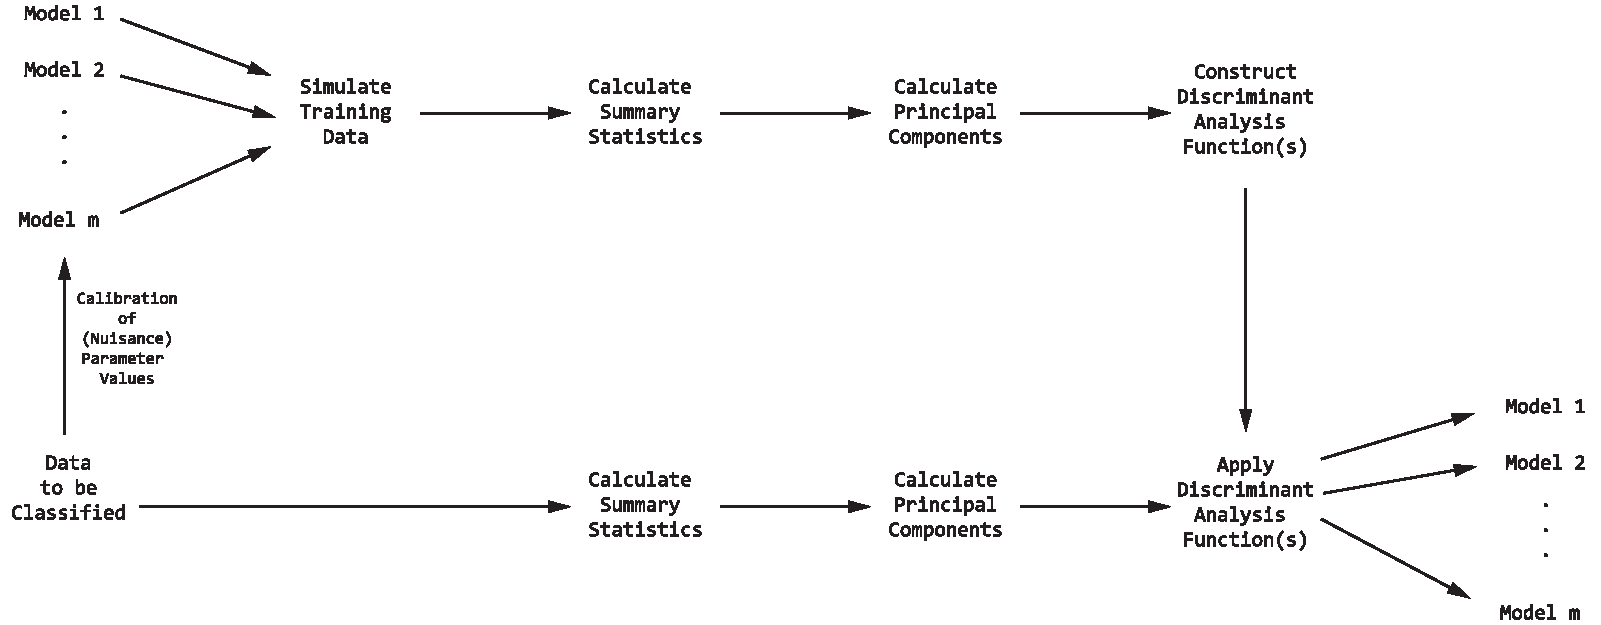
\includegraphics[scale=0.5]{figs/flowchart1.pdf}
        % \caption{default}
        % \label{fig:default}
    \end{center}
\end{figure}

Let $\targetData$ be the \textit{target} data, consisting of an ultrametric phylogeny with each of the tips associated with a geographic range (presence/absence over one or more areas) as well as with set of trait states.
Let $\modelCategories = \{\modelCategory{1}, \modelCategory{2}, ... \modelCategory{k}\}$ be a set of $k$ models that we are interested in studying.
Our analytical objective is, for each $\modelCategory{i}, \modelCategory{i} \in \modelCategories$, estimate the probability that it generated the target data $\targetData$, relative to all the other models in $\modelCategories$.
We achieve this by generating data under each of the models in $\modelCategories$, and then using this \textit{training data} to construct a machine learning classifier, i.e., a discriminant analysis function, that classifies the original data $\targetData$ with respect to each of the models in $\modelCategories$.

\end{document}
